\documentclass[12pt]{article}
\usepackage{graphicx}
\usepackage{amsmath}
%\usepackage{float}
%\usepackage{listings}
\setlength\parindent{0pt} % Removes all indentation from paragraphs

\title{Project - Elevator}
\author{Dominik Koszkul, Michal Oleszczyk, Cezary Dynak, Marek Frydrysiak }
\usepackage{geometry}
\newgeometry{tmargin=2cm, bmargin=2cm, lmargin=2cm, rmargin=2cm}
\begin{document}

\maketitle{}
%\tableofcontents{}


\section{Introduction}
The main goal of the project is to develop an application simulating the behaviour of a lift system. It will consists of a simulator (depicting a state of a set of lifts) and a controller, which will control their activity basing on users requests and the system state.
\newline \\
The main concept is to create two different programs (one for implementation of the controller system and the second one for implementation of the elevators simulation). The programs should be independent, i.e. they should use some general protocol for communication, and work failure-free with any other external programs which also use that specified protocol. Both programs start with a set of parameters: number of elevators and number of floors supported by any of them. The number of floors does not need to be the same for different elevators. Our elevator controller and simulation do not support underground floors.
\newline
\newline
Assumption: at the very beginning all elevators are in the following state: closed doors on the floor 0 (ground floor). The controller remembers current state of all elevators anytime.

\section{Project concept}

\subsection{Module structure}

The module structure of the system is depicted in Figure \ref{fig:DES1}.

\begin{figure}[h!]
  \centering
  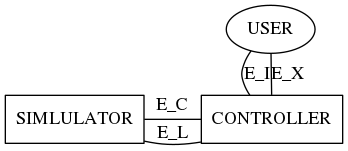
\includegraphics{img/simulator_controller.png}
  \caption{DES graph}
  \label{fig:DES1}
\end{figure}

The system is based on three main parts: the simulator, the controller and the user interface. Essentially, the user interface and the simulator are built within one program. It is as the simulator's part is not only responsible for visualising a state of the lifts, but also it allows a user to interact with it, for instance, by calling a lift on a particular floor choosing a destination floor. 

\subsection{Module communication}

Since the communication protocol between the simulator and the controller is set, it is not necessary for any of them to know how the other works internally. The programs obey the rules of message format, what is sufficiently necessary for a proper communication.
\newline
\newline

The set of events $E$ is described as follows:

\[ E = E^x \cup E^i \cup E^c \cup E^l \]

\begin{enumerate}
\item \textbf{Events from external buttons} 
\[ E^x = [\text{lift\_nr},\text{button\_nr}] \]
\(\text{button\_nr} \in \{\text{button\_down},\text{button\_up}\}\)

\item \textbf{Events from internal buttons}
\[ E^i = [\text{lift\_nr},\text{button\_nr}] \]
\(\text{button\_nr} \in \{0, 1,..., n\}\)

\item \textbf{Events from controller}
\[ E^c = [\text{lift\_nr}, \text{command}] \]
\(\text{command} \in \{\text{go\_down},\text{stop},\text{go\_up},\text{close\_door},\text{open\_door}\}\)

\item \textbf{Events from lifts}
\[ E^l = [\text{lift\_nr}, \text{command}] \]
\(\text{command} \in \{\text{going\_down},\text{stopped},\text{going\_up},\text{closed},\text{opened}\}\)
\end{enumerate}

\section{System model}
\subsection{States}
The state of the system model can be defined as follows:

\[ S = [W, P, Q]. \]
\newline
The sets of states $W$, $P$, $Q$ are precisely explained in the succeeding subsections.

\subsubsection{Lift states}

\[ W=[w_1, w_2, ..., w_i, ..., w_l ]\]
where:
\begin{itemize}
  \item \(l\) - number of lifts
\end{itemize}

\[ w_i = [d_i, o_i, f_i] \]
where:

\(d \in \{\text{going\_down},\text{stopped},\text{going\_up}\}\)

\(o \in \{\text{closed},\text{opened}\}\)

\(f \in \{0,1,...,i,...,n\}\)
\begin{itemize}
  \item \(i\) - next floor to be reached
  \item \(n\) - number of floors
\end{itemize}


\subsubsection{External buttons states}

\[ P = [p_1, p_2, ..., p_i, ..., p_n] \]
where:
\begin{itemize}
  \item \(n\) - number of floors
\end{itemize}

\[ p_i = [g_{i_d}, g_{i_u}] \]
where:\\
\(g_{i_d} \in \{\text{not\_pushed},\text{pushed}\}\)
\(g_{i_u} \in \{\text{not\_pushed},\text{pushed}\}\)\\


\subsubsection{Internal buttons states}
\[ Q = [q_1, q_2, ..., q_i, ..., q_l] \]
where:
\begin{itemize}
  \item \(l\) - number of lifts
\end{itemize}
\[q_i = [b_{i_0}, b_{i_1}, ..., b_{i_j}, ..., b_{i_n}] \]
\(b_{i_j} \in \{\text{not\_pushed},\text{pushed}\} \)

\subsection{Events}


\subsubsection{Events from the external buttons} 
\[ E^x = [\text{lift\_nr},\text{button\_nr}] \]
\(\text{button\_nr} \in \{\text{button\_down},\text{button\_up}\}\)

\subsubsection{Events from the internal buttons}
\[ E^i = [\text{lift\_nr},\text{button\_nr}] \]
\(\text{button\_nr} \in \{0, 1,..., n\}\)

\subsubsection{Events from the lifts}
\[ E^l = [\text{lift\_nr}, \text{command}] \]
\(\text{command} \in \{\text{going\_down},\text{stopped},\text{going\_up},\text{closed},\text{opened}\}\)

\subsection{Transition functions \(f(s,e)\)}

\subsubsection{Events from external buttons}
\[
  f(s_0,[\text{lift\_nr},\text{button\_down}]) =
  [0,[[0,0],...,[g_{\text{lift\_nr}_d}=\text{pushed},0],...,[0,0]],0]
\]
\[
  f(s_0,[\text{lift\_nr},\text{button\_up}]) =
  [0,[[0,0],...,[0,g_{\text{lift\_nr}_u}=\text{pushed},0],...,[0,0]],0]
\]


\subsubsection{Events from internal buttons}
\[
  f(s_0,[\text{lift\_nr},\text{button\_nr}]) =
  [0,[[0,...,0],...,[0,...,b_{\text{lift\_nr}_\text{button\_nr}}=\text{pushed},..,0],...,[0,...,0]],0]
\]

\subsubsection{Events from lifts}
Events from lifts don't change states, they are only information for controller.

\subsection{Initial state \(s_0\)}
All 0.
\[
  s_0 = [0,0,0]
\]

%\section{Automaton description}

%\[ G = (E, S, f, \Gamma, s_0, S_M) \]

\subsection{Marked states \(S_M\)}
All accepted.

\section{Controller model}

\subsection{Events}
\subsubsection{Events from controller}
\[ E^c = [\text{lift\_nr}, \text{command}] \]
\(\text{command} \in \{\text{go\_down},\text{stop},\text{go\_up},\text{close\_door},\text{open\_door}\}\)

\subsection{Transition function\(f(s,e)\)}



\subsubsection{Events from controller}
\(
  f(s_0,[\text{lift\_nr},\text{go\_down}] =
  [[...,[d_\text{lift\_nr}=\text{going\_down},0,f_\text{lift\_nr}+1],...],0,0]
\)\\
\(
  f(s_0,[\text{lift\_nr},\text{stop}] =
  [[...,[d_\text{lift\_nr}=\text{stopped},0,0],...],0,0]
\)\\
\(
  f(s_0,[\text{lift\_nr},\text{go\_up}] =
  [[...,[d_\text{lift\_nr}=\text{going\_up},0,f_\text{lift\_nr}-1],...],0,0]
\)\\
\(
  f(s_0,[\text{lift\_nr},\text{close\_door}] =
  [[...,[0,o_\text{lift\_nr}=\text{closed},0],...],0,0]
\)\\
\(
  f(s_0,[\text{lift\_nr},\text{open\_door}] =
  [[...,[0,o_\text{lift\_nr}=\text{opened},0],...],0,0]
\)



%\subsection{Active event function \(\Gamma(s)\)}
%Active event function \(\Gamma(s)\) corresponde to tansition function\(f(s,e)\).


\section{Implementation}
\subsection{Simulation}
The simulation program was written in the Python2.7 scripting language. For preparation of the user interface we used the $Tkinter$ standard library. 
The simulation consists of 3 modules: graphics.py, elevator.py and my{\_}threads.py. It implements 2 basic classes:  
\begin{itemize}
 \item Stage - class responsible for drawing the user interface in general (makes windows, buttons, digital panels).
 \item Elevator - class responsible for handling the elevator object (sets its parameters, states). 
\end{itemize}
and classes inheriting from the class $Thread$:
\begin{itemize}
 \item MoveLiftDown - class executes command type $X:Y$.
 \item StopLift - class executes command type $X:s$.
 \item MoveLiftUp - class executes command type $X:Y$.
 \item OpenDoors - class executes command type $X:o$.
 \item CloseDoors - class executes command type $X:c$.
 \item ListenInstructions - class listen whether on input port there is any incoming command or not.
 \item SendInstructions - class sends to the output port a command for controller.
\end{itemize}


The program is basing on 4 main threads (to quarantee simultaneously work): 
\begin{itemize}
	\item Main thread - is responsible for the parameters configuration, start other thread and waiting for them to finish.
	\item Graphical thread - is responsible for refreshing the user interface (drawing elevators and floors) and for sending. 
	\item Listenning thread - is responsible for listening on the input port and adding the incoming instructions to the input queue.
	\item Sending thread - is responsible for sending command to the controller via the output port if there is a instruction ready to send in the output queue.		
\end{itemize}

Furthermore, any command read from the controller (like MoveLift, StopLift, OpenDoor, CloseDoor) takes some predefined time. That is why any of that incoming commands starts another independent thread. In that thread, the commands are executed (for example during the MoveLift command the user interface shows direction of movement, highlight a specified floor to green). After the execution that thread puts in the output queue a confirmation of the execution for the controller ($X:a$).
	\begin{figure}
	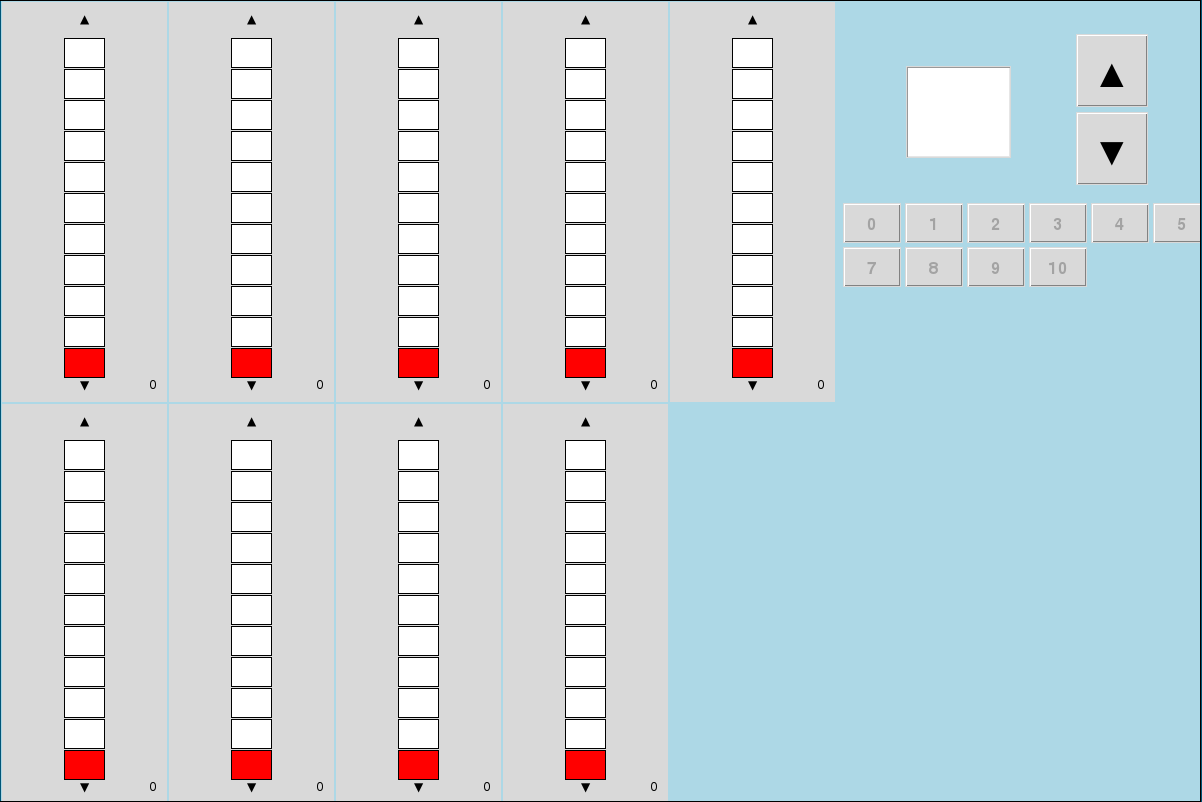
\includegraphics[width=0.93\textwidth]{img/winda.png}
	\end{figure}

\subsection{Controller}
The controller algorithm and program is to be developed.

\subsection{Connection}
The connection is based on simple sockets. The 'incoming' port for the controller is at the same time the 'outcoming' port for the simulation program. On the other hand the outcoming port for the controller is an 'incomming' port for  the simulation.
\newline
\newline
For now:
\newline
controller -\textgreater simulation is realised on port 8089,
\newline
simulation -\textgreater controller is realised on port 8090.

\newpage

\subsection{Protocol}
The protocol corresponds to events defined in previous section.

\subsubsection{Controller \(\to\) Simulation commands}
\begin{enumerate}
	\item $X:Y$ (where X is number of elevator, Y is number of floor) - let elevator X move to floor Y.
	\item $X:s$ (where X is number of elevator) - let elevator X stops.
	\item $X:o$ (where X is number of elevator) - let elevator X opens the door.
	\item $X:c$ (where X is number of elevator) - let elevator X closes the door
\end{enumerate}


\subsubsection{Simulation \(\to\) Controller commands}
\begin{enumerate}
	\item $X:a$ (where X is number of elevator) - elevator X confirms execution of previous controller command.
	\item $Y:d$ (where Y is number of floor) - on the floor Y$^{th}$ user push the button to go down.
	\item $Y:u$ (where Y is number of floor) - on the floor Y$^{th}$ user push the button to go up.
	\item $X:Y$ (where X is number of elevator, Y is number of floor) - inside elevator X user push the button to go to the Y$^{th}$ floor.
\end{enumerate}	

Command $X:a$ should be send from simulation to controller after execution of any controller command. It provides a synchronization between both programs.

\section{Effort}
The task was divided among the group members in the following order:
\begin{enumerate}
\item Michal Oleszczyk - simulation part (main)
\item Dominik Koszkul - simulation part (assistant), documentation
\item Cezary Dynak - controller part (main)
\item Marek Frydrysiak - controller part (assistant), documentation
\end{enumerate}

\end{document}
